A round-robin arbiter is used as the basic arbitration unit in the allocator. The basic structure of the round-robin arbiter is shown in Figure~\ref{fig:rr_arbiter}. The round-robin arbiter used in this design is implemented using a rotating priority pointer and fixed-priority arbitration. The pointer \texttt{ptr} indicates the requester with the highest priority in the current arbitration round. Based on this pointer, the request vector is divided into a masked region and a wrap-around region. The masked request vector is first processed by a fixed-priority arbiter. If no active request exists in the masked region, the original unmasked request vector is arbitrated instead to complete the wrap-around selection.

\begin{figure}[htbp]
    \centering
    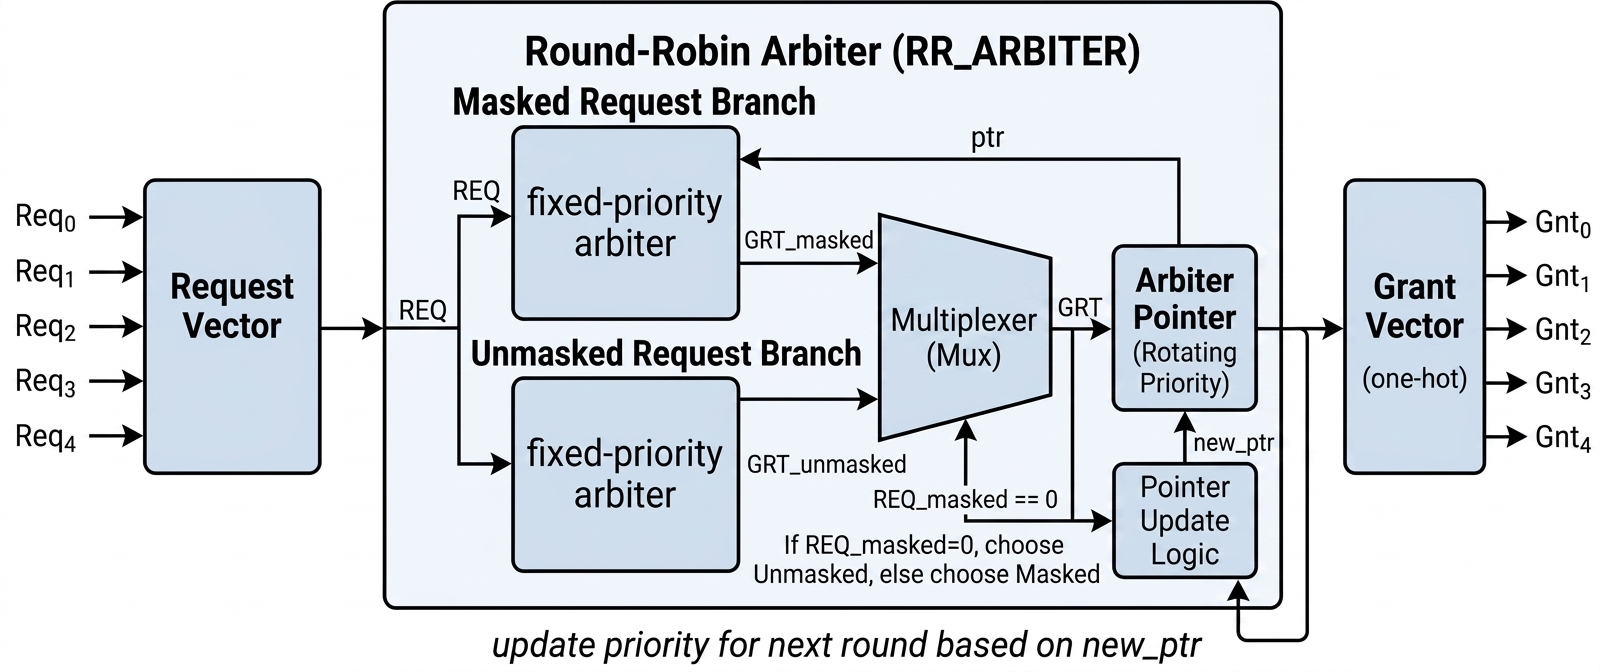
\includegraphics[width=0.85\textwidth]{images/ch3_design_and_implementation/round_robin_arbiter.png}
    \caption{Round-robin arbiter structure}
    \label{fig:rr_arbiter}
\end{figure}

After a grant is generated, the pointer is updated to the requester immediately following the granted one. Therefore, the winning requester is moved to the lowest priority position in the next arbitration round. When arbitration is not enabled or no request is active, the pointer remains unchanged. Compared with a fixed-priority arbiter, this rotating-priority mechanism provides better fairness, prevents one requester from continuously occupying the shared resource, and reduces the possibility of starvation.
